 
An artificial neural network is a network of connected units called neurons or perceptrons, as can be seen in figure \ref{fully_connected}; each arc, which connects two neurons $i$ and $j$, is associated with a weight $w_{ji}$. Perceptrons share the some
structure for all models, what really distinguish a particular model in the family of artificial neural networks is how the perceptron units are arranged and conneceted,for example whether there are cycles
or not, and how data inputs are \textit{fed} to the network. 


\tikzstyle{nn_style}=[->,shorten >=1pt,auto,node distance=1.5cm,
  thick,
  neuron/.style={circle,fill=white!50,node distance=2cm,draw,minimum size=0.7cm,font=\sffamily\normalsize},
  missing/.style={circle,font=\sffamily\Large,node distance=0.95cm},
  label/.style={node distance=1.2cm,rectangle,fill=white!50,draw=none,minimum size=0.7cm,font=\sffamily\normalsize},
  layer/.style={rectangle,fill=white!50,draw,minimum width=1.5cm,font=\sffamily\Large},
  loopStyle/.style={in=120,out=60, distance=2.5cm},
  weight/.style = {above,sloped,pos=0.3},
  thin_edge/.style={line width=0.5pt}]
\begin{figure}
 \centering
\begin{tikzpicture}[nn_style]
   
   \def\layersep{1.5cm}
  
    % Draw the input layer nodes
    \foreach \name / \y in {1,...,4}
    % This is the same as writing \foreach \name / \y in {1/1,2/2,3/3,4/4}
        {\node[neuron] (I-\name) at (\y *1.5,0) {};
        \node[label] (I-\name-label) [below of=I-\name] {$x_\y$};
        }
        
    \foreach \name / \y in {1,...,4}
        \path[->,thin_edge] (I-\name-label)edge[] (I-\name); 

    % Draw the hidden layer nodes
    \foreach \name / \y in {1,...,5}
        \path[yshift=0.5cm,thin_edge]
            node[neuron] (H-\name) at (\y *1.5  -0.9, \layersep) {};

    % Draw the output layer nodes
    \foreach \name / \y in {1,...,3}{
        \path[yshift=0.5cm,thin_edge]
            node[neuron] (O-\name) at (\y *1.5 + 0.6, \layersep*2) {};
         \node[label] (O-\name-label) [above of=O-\name] {$y_\y$};

            }
    \foreach \name / \y in {1,...,3}
        \path[->,thin_edge] (O-\name)edge[] (O-\name-label); 

    % Connect every node in the input layer with every node in the
    % hidden layer.
    \foreach \source in {1,...,4}
        \foreach \dest in {1,...,5}
            \path[thin_edge] (I-\source) edge (H-\dest);
            
    % Connect every node in the hidden layer with every node in the
    % output layer.
    \foreach \source in {1,...,5}
        \foreach \dest in {1,...,3}
            \path[thin_edge] (H-\source) edge (O-\dest);

\end{tikzpicture}
\caption{Artificial neural network example}
\label{fully_connected}
\end{figure}


As you can see in figure \ref{neuron_model} each neuron is \textit{fed} with a set inputs which are the weighted outputs of other neurons and/or other external inputs.
Formally the output of a perceptron $\phi_j$
is defined as:
 
\begin{align}
&\phi_j \triangleq \sigma(a_j)\\
&a_j \triangleq \sum_l w_{jl}\phi_l +b_j
\end{align}

where $w_{jl}$ is the weight of the connection between neuron $l$ and neuron $j$, $\sigma(\cdot)$ is a non linear function and $b_j \in \mathbb{R}$ is called bias.
It's worth noticing that in this formulation the input $\phi_l$ can be the outputs of other neurons or provided external inputs.


\tikzstyle{nn_style}=[->,shorten >=1pt,auto,node distance=1.5cm,
  thick,
  neuron/.style={circle,fill=white!50,node distance=1cm,draw,minimum size=0.7cm,font=\sffamily\normalsize},
  missing/.style={circle,font=\sffamily\Large,node distance=0.95cm},
  label/.style={node distance=1.2cm,rectangle,fill=white!50,draw=none,minimum size=0.7cm,font=\sffamily\normalsize},
  layer/.style={rectangle,fill=white!50,draw,minimum width=1.5cm,font=\sffamily\Large},
  loopStyle/.style={in=120,out=60, distance=2.5cm},
  weight/.style = {above,sloped,pos=0.3},]
\begin{figure}
 \centering
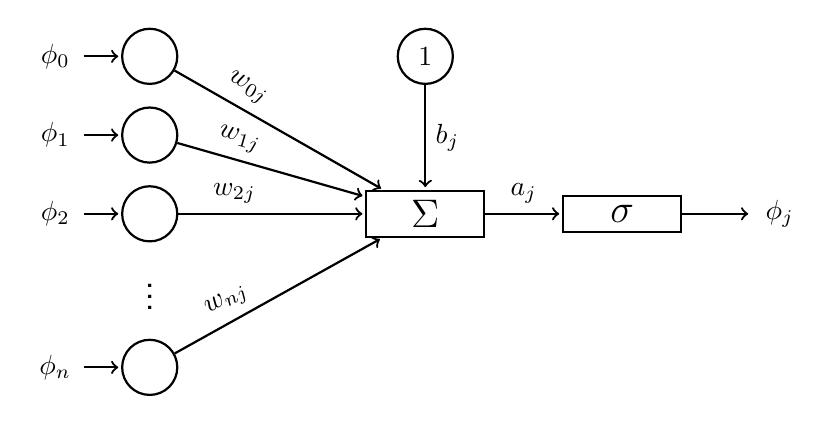
\begin{tikzpicture}[nn_style]

  \node[neuron]    (x0)       {};
  \node[neuron]    (x1)[below of=x0]   {};
  \node[neuron]    (x2)[below of=x1]   {};
  \node[missing]   (x3)[below of=x2]   {$\vdots$};
  \node[neuron]    (xn)[below of=x3]   {};
  
  
  \node[label]    (u0)[left of=x0]   {$\phi_0$};
  \node[label]    (u1)[left of=x1]   {$\phi_1$};
  \node[label]    (u2)[left of=x2]   {$\phi_2$};
  \node[label]    (un)[left of=xn]   {$\phi_n$};
  
  
  \node[layer] (hl)[ right of=x2,node distance=3.5cm] {$\Sigma$};
  \node[neuron](bias)[above of=hl,node distance=2cm]{$1$};
  \node[layer] (ol)[right of=hl,node distance=2.5cm] {$\sigma$};
  
  \node[label]  (phi)[right of=ol,node distance=2cm] {$\phi_j$};
   
  
  \path[->] (x0) edge [] node[weight]{$w_{0j}$}   (hl)
	    (x1) edge [] node[weight]{$w_{1j}$}   (hl)
	    (x2) edge [] node[weight]{$w_{2j}$}   (hl)
	    (xn) edge [] node[weight]{$w_{nj}$}   (hl)
 	    (bias) edge[]  node[]{$b_{j}$}(hl)
	    (u0) edge []   (x0)
	    (u1) edge []   (x1)
	    (u2) edge []   (x2)
	    (un) edge []   (xn)
	    (hl) edge []   node[]{$a_{j}$}(ol)
	    (ol) edge []   (phi);

\end{tikzpicture}
\caption{Neuron model}
\label{neuron_model}
\end{figure}

\paragraph{The activation function}
The $\sigma$ function is called \textit{activation} function and should determine wheter a perceptron unit is \textit{active} or not. When artificial neural networks where first conceived, back in 80es,
trying to mimic the brain structure, such function was a simple threshshold function, trying to reproduce the behaviour of brain neurons: a neuron is \textit{active}, i.e it's output $\phi_j$ is $1$, if
the input stimuli $\sum_l w_{jl}\phi_l +b_j$ are greater than a given threshold $\tau$.

\begin{equation}
  \sigma_{\tau}(x)=\begin{cases}
    1 & \text{if $x>\tau$}.\\
    0 & \text{otherwise}.
  \end{cases}
\end{equation}

Such function, however, is problematic when we are to compute gradients because it's not continuoos, so one of the following function is usually choosen:

\begin{equation}
 sigmoid(x)=\frac{1}{1+e^{-x}}
\end{equation}
\begin{equation}
 tanh(x)=\frac{e^x-e^{-x}}{e^x+e^{-x}}
\end{equation}
These functions behave similarly to the threshold function, but, because of their \textit{smoothness}, present no problems in computing gradients.

Another function which is becoming a very popular choice is the \textit{rectified linear unit}:
\begin{equation}
  ReLU(x)=\begin{cases}
    x & \text{if $x>0$}.\\
    0 & \text{otherwise}.
  \end{cases}
\end{equation}
ReLU activation function is rather different from previous activation functions, some of these difference, in particular with respect to gradients will be analyzied in later sections.

It's worth noticing that the activation function it's the only component which make artifical neuron networks a non linear model. Were we to choose a \textit{linear} function as activation funciont we will
end up with a simple linear model since the outputs of the network would be ultimately composed only of sums and products.

\paragraph{The bias term}
Let's consider the old threshold function $\sigma_{\tau}$, and ask ourselves what the bias term is for, what does changing this term bring about.
Suppose neuron $j$ if fed with inputs $a_j = \sum_l w_{jl}\phi_l$; if $a_j>\tau$ that neuron is active otherwise it is not. Now, let's add the bias term to $a_j$;
we obtain that neuron $j$ is active if $a_j>\tau-b_j$. So the effect of the bias term is to change the activation threshold of a given neuron. Using bias terms in a neural network architecture gives us
the ability to change the activation threshold for each neuron; that's particularly important considering that we can learn such bias terms.
We can do these same considerations in an analogous way for all the other activation funcitons.
\\\\
It's often useful to think of a neurual network as series of layers, one on top of each other, as depicted in figure \ref{layered_nnet}. The first layer is called the input layer and its units are \textit{fed}
with external inputs, the upper layers are called \textit{hidden layers} because their's outputs are not observed from outside except the last one which is called \textit{output layer} because it's output 
is the output of the net.

Whene we describe a network in this way is also useful to adopt a different notation: we describe the weights of the net with a set of matrixes $W_i$ one for each layer, and neurons are no more
linearly indexed, insted with refer to a neuron with a relative index with respect to the layer; this allows to write easier equations in matrix notation
\footnote{In the rest of the book we will refer to the latter notation as \textsl{matrix notation} and to the previous one as \textsl{linear notation}}.


\tikzstyle{rnn_style}=[->,shorten >=1pt,auto,node distance=1.5cm,
  thick,
  neuron/.style={circle,fill=white!50,draw,node distance = 1cm, minimum size=0.7cm,font=\sffamily\Large\bfseries},
  missing/.style={rectangle,fill=white!50,node distance =1cm,draw=none,minimum size=0.7cm,font=\sffamily\Huge\bfseries},
  label/.style={node distance=1.2cm,rectangle,fill=white!50,draw=none,minimum size=0.7cm,font=\sffamily\normalsize},
  layer/.style={rectangle,fill=white!50,draw,minimum width=4cm,font=\sffamily\normalsize},
  loopStyle/.style={in=120,out=60, distance=2.5cm},]
\begin{figure}
 \centering
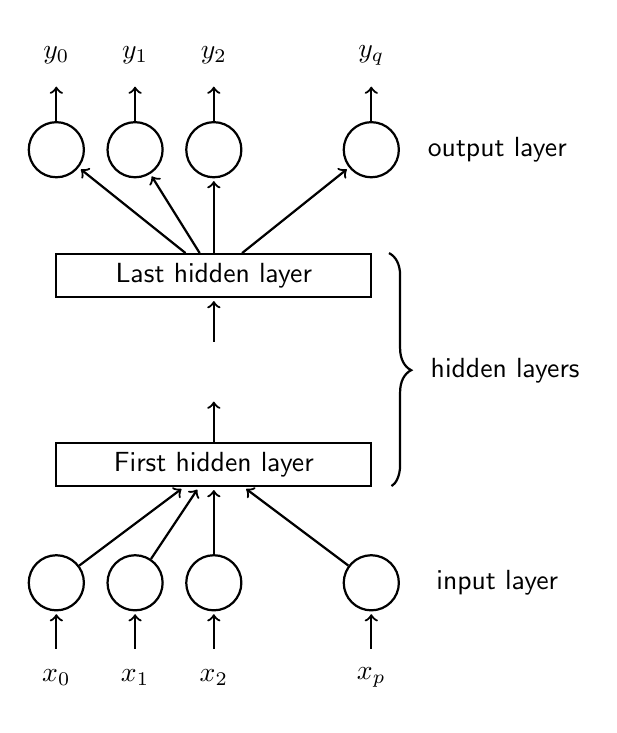
\begin{tikzpicture}[rnn_style]

  \node[neuron]    (x0)       {};
  \node[neuron]    (x1)[right of=x0]   {};
  \node[neuron]    (x2)[right of=x1]   {};
  \node[missing]   (x3)[right of=x2]   { $\hdots$};
  \node[neuron]    (xn)[right of=x3]   {};
  
  \node[label]    (u0)[below of=x0]   {$x_0$};
  \node[label]    (u1)[below of=x1]   {$x_1$};
  \node[label]    (u2)[below of=x2]   {$x_2$};
  \node[label]    (un)[below of=xn]   {$x_p$};
  
  

    
  \node[layer] (hl)[above of=x2,node distance=1.5cm] {First hidden layer};
  \node[missing] (hls)[above of=hl,node distance=1.2cm]{$\hdots$};
  \node[layer] (ol)[above of=hls,node distance=1.2cm] {Last hidden layer};
  
  \draw[decorate,decoration={brace,raise=6pt,amplitude=8pt}, thick,-]
   (ol.north east)--(hl.south east);



  
  \node[neuron] (o1) at (0,5.5) {};
  \node[neuron] (o2)[right of=o1] {};
  \node[neuron] (o3)[right of=o2] {};
  \node[missing](o4)[right of=o3] {$\hdots$};
  \node[neuron] (on)[right of=o4] {};
  
  
  \node[label]    (y0)[above of=o1]   {$y_0$};
  \node[label]    (y1)[above of=o2]   {$y_1$};
  \node[label]    (y2)[above of=o3]   {$y_2$};
  \node[label]    (yn)[above of=on]   {$y_q$};
  
     
  \node[label]    (hls_label)[right of=hls,node distance=3.7cm]   {hidden layers};
  \node[label]    (input_label)[right of=xn,node distance=1.6cm]   {input layer};
  \node[label]    (output_label)[right of=on,node distance=1.6cm]   {output layer};
  
  
  \path[->] (x0) edge [] node[]{}   (hl)
	    (x2) edge []   (hl)
	    (x1) edge []   (hl)
	    (xn) edge []   (hl)
	    (u0) edge []   (x0)
	    (u1) edge []   (x1)
	    (u2) edge []   (x2)
	    (un) edge []   (xn)
	    (ol) edge []   (o1)
	    (ol) edge []   (o2)
	    (ol) edge []   (o3)
	    (ol) edge []   (on)
	    (o1) edge []   (y0)
	    (o2) edge []   (y1)
	    (o3) edge []   (y2)
	    (on) edge []   (yn)
	    (hl) edge []  node[]{} (hls)
	    (hls) edge []  node[]{} (ol);


\end{tikzpicture}
\caption{Layered structure of an artificial neural network}
\label{layered_nnet}
\end{figure}